% \chapter{Methods}
% \label{chapter:methods}

%%% SECTION
\section{Introduction}
%\subsection{Introduction}
As described in the project objectives, this study aims to find similarities between the gene expression regulated by Cyclin D1 in MCL and the gene expression of the DDR, using Data Mining and Machine Learning techniques combined with Statistical Tests and biological analysis, to identify the significant enriched genes that can act as therapeutic target and biomarkers.

In order to fulfill these goals, this study has been developed following two different approaches that share a common part on the data cleaning and the final GSEA process, but differ on the data normalization and posterior gene selection processes. The following sections will explain in details the two scenarios, but before going into details, it is worth to mention that two public data sets from Gene Expression Omnibus repository (GEO) were selected for this study. These data sets are:

\begin{itemize}
    \item GSE25848 \cite{ddrData:2011}: which contains data about DDR.
    \item GSE21452 \cite{mclData:2011}: which contains data from MCL tumors.
\end{itemize}

\newpage
\section{Scenario 1}

The first developed pipeline is described in the following figure.

\begin{figure}[h]
    \centering
    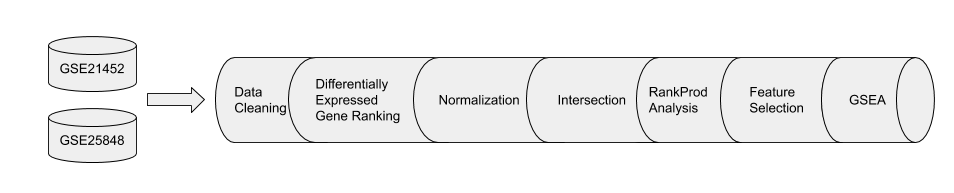
\includegraphics[scale=0.5]{../figs/scenario_1_figure.png}
    \caption{Scenario 1 pipeline}
    \label{fig:scenario-1}
\end{figure}

As seen in the figure, the pipeline is composed by seven steps or sub-processes:

\begin{itemize}
    \item \textbf{Data cleaning:} the data from the two original data sets are cleaned and prepared for the posterior steps.
    \item \textbf{Differentially expressed gene ranking:} A first ranking of genes is generated. This ranking is done per each individual data set.
    \item \textbf{Normalization:} process to allow the posterior merge of both data sets.
    \item \textbf{Intersection:} Common genes from both data sets are discovered and merged into a new data set.
    \item \textbf{RankProd analysis:} common genes are analyzed in order to find up and down regulated genes.
    \item \textbf{Feature selection:} machine learning algorithms are applied to find the most important features (genes).
    \item \textbf{GSEA:} analysis to find significantly enriched genes.
\end{itemize}

\subsection{Data Cleaning}
The first step in the pipeline consist on a general inspection of the data sets and the posterior data cleaning process. This data cleaning process consisted mainly in removing the entries containing empty or \textit{NA} values.

\subsection{Differentially Expressed Gene Ranking}

A first selection of genes was done in this step. The purpose of this selection is to get the top ten thousand differentially expressed genes from each of both data sets.
This process was done using the multiClust\cite{multiClust} package in R/Bioconductor.

As a result of this step, two new data sets were created. Each of these data sets were composed by ten thousand of the most differentially expressed genes of its parent data set. 

\subsection{Normalization}
Once the previous steps were performed, a normalization process was applied to the new created (and reduced) data sets. In this case, a log2 transformation was applied to the data coming from the data set GSE25848. The data contained in GSE21452 was kept as it was, due to the fact that it was already log2 transformed.

Thanks to this transformation, the data coming from both data sets were in a similar scale, and able to be merged.

\subsection{Intersection}

During this process, a match between the two new reduced data sets was performed, and as a result, a new data set containing only the matched genes was created. This new data set is the one that will be used for the posterior analysis, but before passing to the next step, another data cleaning process was performed. In this case, some \textit{NA} values were generated after the log2 transformation, and they needed to be removed. Also, the name of the genes were reviewed in order to ensure that they were valid for the upcoming steps.

\subsection{RankProd Analysis}
The following step in the pipeline is the identification of up-regulated and down-regulated genes in our data set. For that purpose, a RankProd analysis was performed using the Bioconductor package RankProd. 

As a result of this process, 262 up-regulated genes and 268 down-regulated genes were selected. This selection was done using a cut off value of 0.05 on the p-values.

\subsection{Feature Selection}
Once the up-regulated and down-regulated genes were identified, a Feature Selection process was carried out. 
A Random Forest method was applied as an Unsupervised Feature Selection method.
As a consequence, a list of features sorted by importance was generated. From that list, the top 20 features identified by the algorithm were collected. This identification was done for both, the up and down regulated genes.

\subsection{GSEA}
As a final step, two different ways of executing a GSEA were carried out.
First, the Bioconductor package FGSEA\cite{fgsea} was used, but the results of this process were not satisfactory.
After that first attempt, the original GSEA method\cite{Subramanian15545} was performed, but again, with unsatisfactory results, where no significantly enriched genes were obtained.

This negative results forced the re-design of the experiment, and the second scenario was designed.

\newpage
\section{Scenario 2}

For this second attempt, the focus was placed in the correlation between gene expressions and the Cyclin D1 expression.

The complete pipeline is represented in the next figure.

\begin{figure}[h]
    \centering
    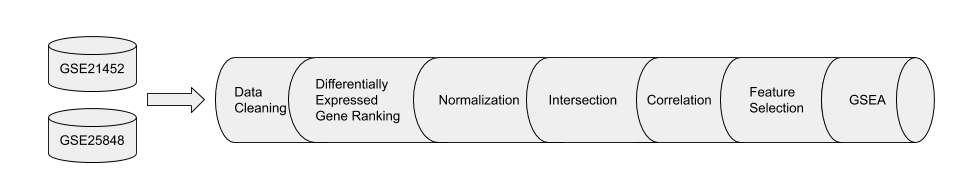
\includegraphics[scale=0.5]{../figs/scenario_2_figure.png}
    \caption{Scenario 2 pipeline}
    \label{fig:scenario-2}
\end{figure}

As seen in the figure, the pipeline is composed by similar sub-processes to the previous pipeline from scenario 1. The main difference in this one is the different normalization applied and the substitution of the RankProd analysis by the correlation analysis.

The first two steps from the previous scenario (data cleaning and differentially expressed gene ranking) were shared with this one, therefore, this scenario starts with an already existing ranked list of ten thousand genes per data set, which was obtained at the end of the Differentially Expressed Gene Ranking process. Due to that fact, the detailed explanation of these two sub-processes are going to be skipped in the following paragraphs.


\subsection{Normalization}
The third step in the pipeline is a normalization process. The main goal was to transform the data from both data sets to the same scale.
Such transformation allowed the integration and correlation of data from both data sets.

The normalization applied in this case was a z-scored normalization.

\subsection{Integration}
The integration of the two data sets was carried out in a similar way than the one executed in the scenario 1.
As a result, a new data set with the common genes is obtained.

The difference between this one and the one generated in the first scenario is that in this one, the data has suffered a different normalization, and therefore, the \textit{NA} values that were generated in the log2 transformation are not present, which means that fewer data had to be removed.

\subsection{Correlation with Cyclin D1}
Continuing with this second pipeline, the next step was the calculation of the correlation between the expression of the available genes and the expression of Cyclin D1.

Once this correlation was calculated, a K-Means algorithm was applied.
The purpose of running this method was to create 3 clusters and classify the data into three different types of correlation: positive correlation, no significant correlation and negative correlation.

At the end of this correlation process, two new columns were added to the data set, the first one containing the correlation value of each gene and the second one with the cluster where each gene belongs.

Because of time constrains, only the genes in the positive correlation cluster were studied in the following steps, keeping for future studies the possibility to run GSEA with the negative correlation cluster.

As a result, a 316 genes were selected for the next step.

\subsection{Feature Selection}
Similar to the Feature Selection process in the previous pipeline, a Random Forest algorithm was executed. Again, as in the previous scenario, the Random Forest method was applied in an unsupervised way, giving as a result a list of features (genes) ranked by importance.
From that list of ranked genes, 205 were selected to be passed to the final GSEA process. This number was chosen to ensure that the Cyclind D1 (CCND1) was contained in that selection.

\subsection{GSEA}

As a final step, a GSEA process was carried out.
GSEA takes as input a molecular profile data set and a gene set database.
The selection of genes obtained in the Feature Selection process was passed as first input. The gene set database used in this process was obtained from MSigDB. That database is the C6, which contains data from oncogenic gene sets. These gene sets were defined directly from microarray gene expression data from cancer gene perturbations.

Is important to mention the phenotype argument used for the GSEA process.
As this study focuses on Cyclin D1, its corresponding gene was selected to be used as phenotype, in that way, a correlation with this gene was used.

The result of running GSEA on those inputs were that four up-regulated gene sets were identified as significantly enriched at nominal p-value smaller than 0.05, and 3 down-regulated gene sets were identified as significantly enriched at nominal p-value smaller than 0.05.

\section{Future Developments}

One of the purposes of this study was to include more Feature Selection algorithms in the pipelines, but due to the lack of time this objective is left for future improvements.

The idea of integrating more than one Feature Selection algorithm was to execute several of them in parallel and combine their results. This combination can be done matching the common genes that are selected by each algorithm and perform GSEA over that new set of genes.

Another improvement can be the usage of Supervised methods of Feature Selection. This Supervised method can be done adding a new vector of labels. This labels can be \textit{MCL} and \textit{DDR} and can be associated to the samples that comes from the MCL dataset and the DDR data set respectively.